\documentclass[10pt, a4paper]{article}

\usepackage{geometry}
\usepackage{amsmath}
\usepackage{graphicx}
\usepackage{booktabs}

\title{\textbf{HW1 - Classification trees, random forests}}
\author{Vanja Stojanovi\'c}
\date{March 2026}

\begin{document}
\maketitle

\section{CART and Random Forests}

Each prediction is a Bernoulli trial (correct or not).
For misclassification rate $\hat{p}$ on $n$ samples:
\[
    SE = \sqrt{\frac{\hat{p}(1 - \hat{p})}{n}}
\]

\subsection{Classification Tree}

Full tree with \texttt{min\_samples=2}:

\begin{table}[ht!]
\centering
\begin{tabular}{lcc}
\toprule
Dataset & Misclassification rate & SE \\
\midrule
Train & 0.000 & 0.000 \\
Test  & 0.267 & 0.057 \\
\bottomrule
\end{tabular}
\end{table}

\subsection{Random Forest}

Random forest with $n=100$ trees, \texttt{min\_samples=2}:

\begin{table}[ht!]
\centering
\begin{tabular}{lcc}
\toprule
Dataset & Misclassification rate & SE \\
\midrule
Train & 0.000 & 0.000 \\
Test  & 0.233 & 0.055 \\
\bottomrule
\end{tabular}
\end{table}

\subsection{Misclassification Rate vs Number of Trees}
Graph shown in Fig. \ref{fig:rate_vs_num_trees}.
\begin{figure}[ht!]
\centering
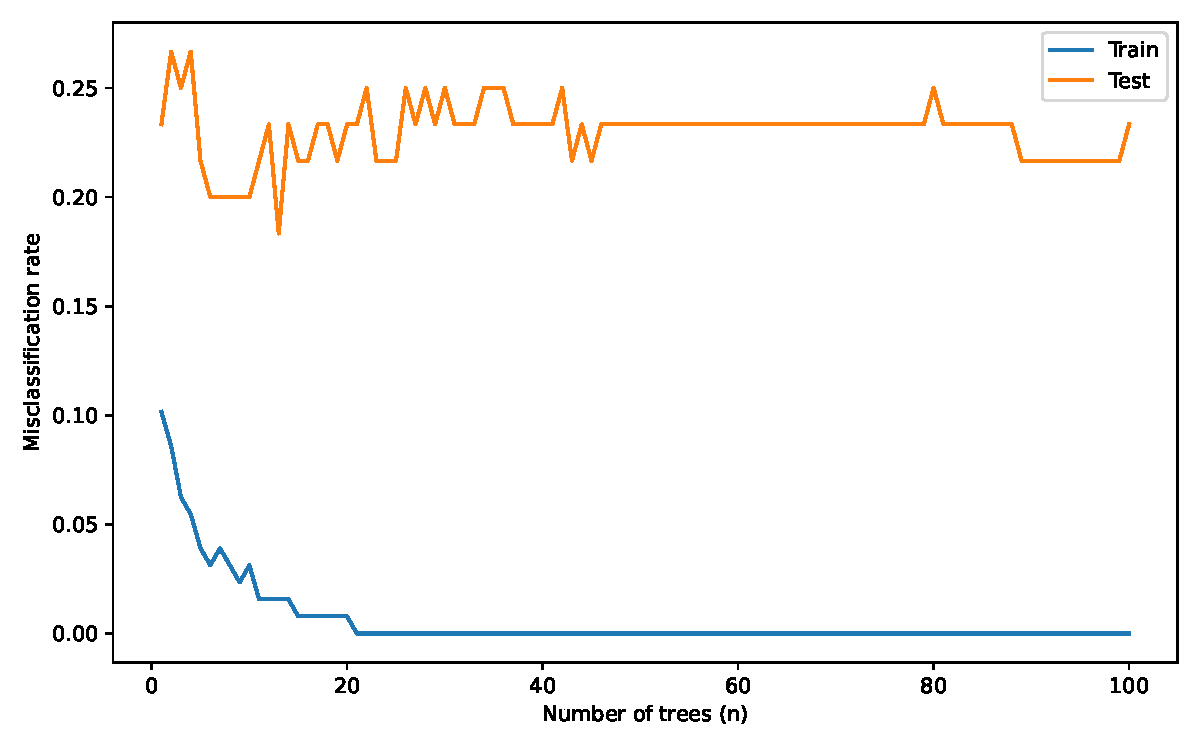
\includegraphics[width=0.8\textwidth]{misclassification_vs_n.pdf}
\caption{Misclassification Rate vs Number of Trees}
\label{fig:rate_vs_num_trees}
\end{figure}

\section{Variable Importance}

Permutation-based importance: for each tree, the OOB (out-of-bag) accuracy is computed,
then each feature is permuted in the OOB samples and accuracy is recomputed.
The drop in accuracy averaged over all trees gives the feature's importance. The graph is shown in Fig. \ref{fig:importance}.

\begin{figure}[ht!]
\centering
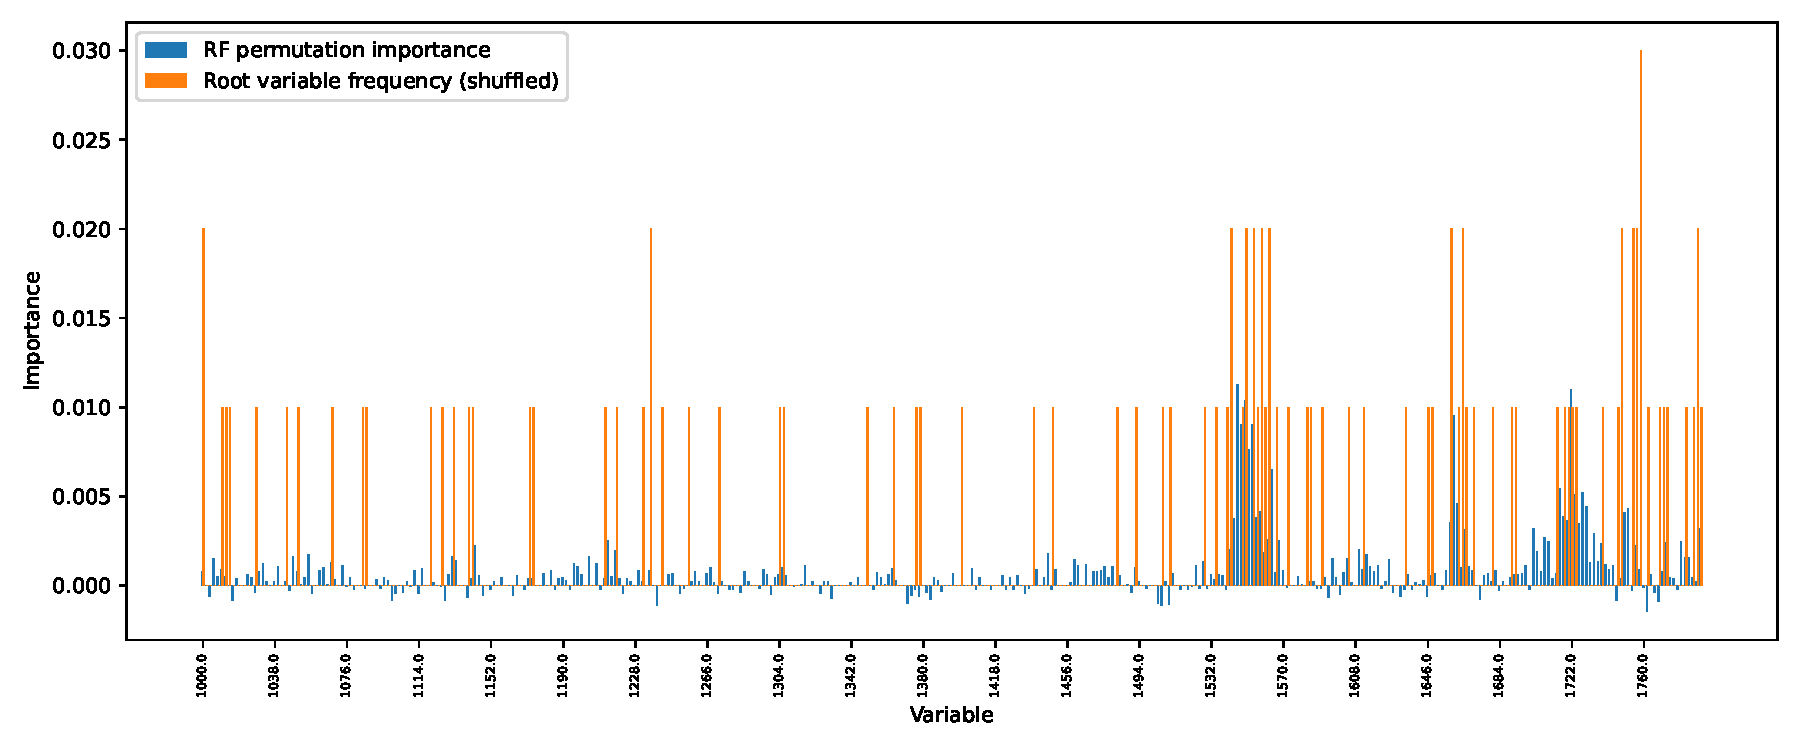
\includegraphics[width=0.8\textwidth]{importance.pdf}
\caption{Variable importance}
\label{fig:importance}
\end{figure}

\section{Improved Trees}

All results below use 10-fold cross-validation on the combined train+test data (188 samples).

\begin{table}[ht!]
\centering
\begin{tabular}{lcc}
\toprule
Method & CV error & SE \\
\midrule
Tree (\texttt{min\_samples=2}) & 0.208 & 0.022 \\
BetterTree (\texttt{min\_samples=5}) & 0.197 & 0.024 \\
BetterTree2 (PCA, 20 components) & 0.227 & 0.029 \\
\bottomrule
\end{tabular}
\end{table}

\subsection{BetterTree: Pre-pruning}

The full tree with \texttt{min\_samples=2} achieves 0\% training error but 20.8\% CV error,
indicating overfitting. With 396 features and only $\sim$170 training samples per fold,
the tree can always find a feature that perfectly separates a small node---even when that
split captures noise rather than signal. Increasing \texttt{min\_samples} to 5 prevents the
tree from creating leaves with very few samples, forcing it to generalize.
This yields a modest but consistent improvement (19.7\% vs 20.8\%).

We also tested cost-complexity pruning (CART's standard post-pruning) and reduced error
pruning, but both performed worse. Cost-complexity pruning requires nested CV for
$\alpha$ selection, which is unreliable with only $\sim$170 samples. Reduced error pruning
wastes 20\% of already scarce data on a validation split. On small datasets, the simplest
regularization (larger \texttt{min\_samples}) outperforms more sophisticated but data-hungry
pruning strategies.

\subsection{BetterTree2: PCA + tree (negative result)}

FTIR spectra have highly correlated adjacent features, making PCA a natural
preprocessing step. However, PCA projects onto directions of maximum variance,
which may not align with the directions most discriminative for classification.
Trees split on individual features, and PCA components are dense linear combinations
of all features---this mismatch means PCA can obscure the sharp spectral peaks that
a tree would otherwise exploit. Performance degraded across all tested component
counts (3--50), confirming that for tree-based classifiers on spectral data,
retaining the original feature space is preferable.

\subsection{Trade-offs}

The fundamental limitation is that a single decision tree cannot escape the
bias-variance trade-off: with few samples and many features, either the tree
overfits (low \texttt{min\_samples}) or underfits (high \texttt{min\_samples}).
The random forest's advantage---averaging over diverse trees---is the principled
solution, which is why it consistently outperforms any single-tree approach on this data.

\end{document}
